%--------------------------------Dependencies----------------------------------%
%   amssymb                                                                    %
%   pgfplots                                                                   %
%       compat=1.9                                                             %
%   tikz                                                                       %
%       arrows.meta                                                            %
%   Unary minus sign.                                                          %
%       \DeclareMathSymbol{\minus}{\mathbin}{AMSa}{"39}                        %
%-------------------------------Main Document----------------------------------%

%-----------------------------------LICENSE------------------------------------%
%   This file is part of Mathematics-and-Physics.                              %
%                                                                              %
%   Mathematics-and-Physics is free software: you can redistribute it and/or   %
%   modify it it under the terms of the GNU General Public License as          %
%   published by the Free Software Foundation, either version 3 of the         %
%   License, or (at your option) any later version.                            %
%                                                                              %
%   Mathematics-and-Physics is distributed in the hope that it will be useful, %
%   but WITHOUT ANY WARRANTY; without even the implied warranty of             %
%   MERCHANTABILITY or FITNESS FOR A PARTICULAR PURPOSE.  See the              %
%   GNU General Public License for more details.                               %
%                                                                              %
%   You should have received a copy of the GNU General Public License along    %
%   with Mathematics-and-Physics.  If not, see <https://www.gnu.org/licenses/>.%
%------------------------------------------------------------------------------%

% Use the standalone class for displaying the tikz image on a small PDF.
\documentclass[crop, tikz]{standalone}

% Import the tikz and pgfplots packages to use for the drawing.
\usepackage{tikz, pgfplots}

% Needed of blackboard bold C and unary minus sign.
\usepackage{amssymb}

% Unary minus sign.
\DeclareMathSymbol{\minus}{\mathbin}{AMSa}{"39}

% The arrows package is used for the LaTeX arrow.
\usetikzlibrary{arrows.meta, decorations.markings}

% Begin the document.
\begin{document}

    % Draw the figure.
    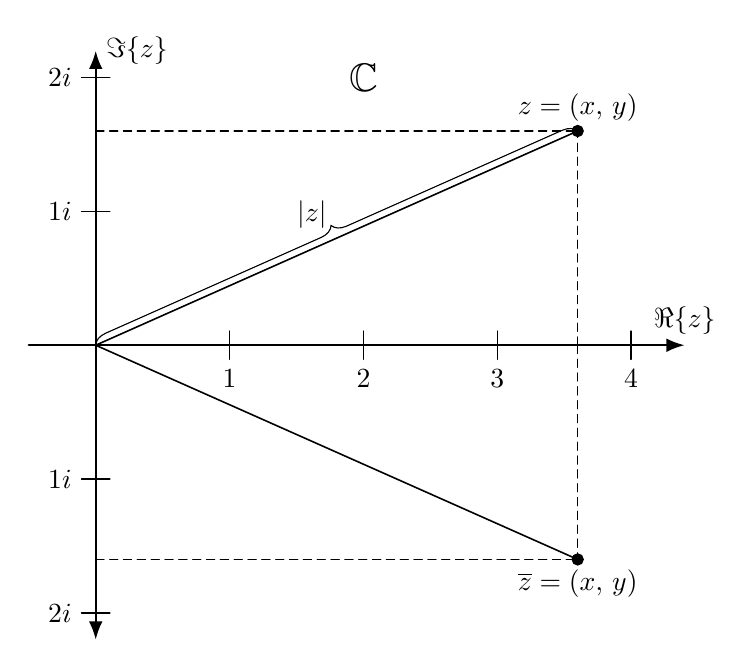
\begin{tikzpicture}[%
        >=Latex,
        line width=0.2mm,
        line cap=round,
        scale=1.7
    ]

        % Coordinates for the various points used.
        \coordinate (O)       at (0.0,  0.0);
        \coordinate (z_x)     at (3.6,  0.0);
        \coordinate (z_y)     at (0.0,  1.6);
        \coordinate (z)       at (3.6,  1.6);
        \coordinate (z_bar)   at (3.6, -1.6);
        \coordinate (z_bar_y) at (0.0, -1.6);
        \coordinate (C)       at (2.0,  2.0);

        % Axes:
        \begin{scope}[thick]
            \draw[->]  (-0.5,  0.0) to (4.4, 0) node [above] {$\Re\{z\}$};
            \draw[<->] ( 0.0, -2.2) to (0, 2.2) node [right] {$\Im\{z\}$};
        \end{scope}

        % Axes labels:
        \foreach\n in {1, 2}{%
            \draw (\n, 3pt)  to (\n, -3pt)  node [below] {$\n$};
            \draw (3pt, \n)  to (-3pt, \n)  node [left]  {$\n{i}$};
            \draw (3pt, -\n) to (-3pt, -\n) node [left]  {$\minus\n{i}$};
        }

        % More labels for the x-axis.
        \foreach\n in {3, 4}{%
            \draw (\n, 3pt) to (\n, -3pt) node [below] {$\n$};
        }

        % Draw a line from the origin to the point (x, y).
        \draw (O) to node [above left] {$|z|$} (z);

        % Draw a brace denoting the magnitude of z.
        \draw[decorate, decoration={brace, amplitude=5pt},thin] (O) to (z);

        % Draw a line from the origin to the conjugate of z.
        \draw (O) to (z_bar);

        % Scope for dashed lines.
        \begin{scope}[densely dashed, thin]
            % Draw dashed lines for z.
            \draw[densely dashed, thin] (z_y) to (z);
            \draw[densely dashed, thin] (z_x) to (z);

            % Draw dashed lines for the conjugate of z.
            \draw[densely dashed, thin] (z_bar_y) to (z_bar);
            \draw[densely dashed, thin] (z_x)     to (z_bar);
        \end{scope}

        % Points for z and z_bar.
        \draw[fill=black] (z)     circle (0.4mm);
        \draw[fill=black] (z_bar) circle (0.4mm);

        % Nodes for labelling.
        \node at (C)              {\Large{$\mathbb{C}$}};
        \node at (z)     [above]  {$z=(x,\,y)$};
        \node at (z_bar) [below]  {$\overline{z}=(x,\,\minus{y})$};
    \end{tikzpicture}
\end{document}
